% Add two graphs ( design.py ) after Spectral Equation Slide
\documentclass{beamer}
\usepackage[style=authoryear, backend=biber]{biblatex}
\addbibresource{citations.bib}
\usepackage{graphicx}
\usepackage{tikz}
\usetikzlibrary{shapes, arrows}
\title{Using Simultaneous Perturbation Stochastic Approximation to Design a Three-String Network With Strictly Odd-Harmonics}
\author{Srinivas Vadhiraj (Mentor: Saba Goodarzi)}
% \date{August 3, 2023}

\begin{document}
\frame{\titlepage}
% Todo : Table of Contents ( outline )
\begin{frame}
\frametitle{Overview}
\begin{columns}[t]
\column{0.5\textwidth}
\begin{enumerate}
\item Introduction to Acoustics
\item Different Kinds of Instruments
\item String Networks
\end{enumerate}
\column{0.5\textwidth}
\begin{enumerate}
\setcounter{enumi}{3}
\item Optimization
\item Results
\item What's Next?
\end{enumerate}
\end{columns}
\end{frame}

%% FRAME 1: SOUND
%% My talk is about designing musical instruments -> I am going to talk about sound first as it is important.
\begin{frame}
\frametitle{Visually Representing Sound}
    \centering
    \begin{figure}
    \includegraphics[width=\textwidth,height=.8\textheight,keepaspectratio]{diagram.png}
    \caption{Waveform Representation of Sound and its Properties}
    \end{figure}
\end{frame}


% FRAME 2: Decomposing Complex Waveforms
%% Bullet 1: Fourier Series
%% Bullet 2: Fourier Transform 
\begin{frame}
\frametitle{Waveforms Can be Represented as the Sum of Sinusoidal Functions}
    \centering
    \begin{figure}
    \includegraphics[width=\textwidth,height=.8\textheight,keepaspectratio]{decomposing_wave.png}
    \caption{Fourier Series Decomposing a Waveform}
    \end{figure}
\end{frame}


%%Frame 3: The Spectrum
%% 
% Bullets: Fundamental Frequency
%%PArtials 
%% Harmonic vs. Inharmonic Spectrum
\begin{frame}
\frametitle{Spectrum}
    \centering
    \begin{figure}
    \includegraphics[width=\textwidth,height=.8\textheight,keepaspectratio]{spectrum.png}
    \caption{Fundamental Frequency and Overtone/Partial Ratio Spectrum}
    \end{figure}
\end{frame}


\begin{frame}
  \centering
  \Huge\textbf{Different Kinds of Instruments}
\end{frame}
\begin{frame}{Harmonic Instruments}
    \begin{columns}
        \column{0.5\textwidth}
        \begin{figure}
            \includegraphics[width=\textwidth]{string.png}
            \caption{Uniform Musical String}
        \end{figure}
        
        \column{0.5\textwidth}

        
        \vspace{1cm}
                \textbf{Resonant Frequencies:}
                % \begin{align*}
                $\Omega &= \{f_0, 2f_0, 3f_0, 4f_0, \ldots \} \\$
                % \intertext{Where $f_0$ is the fundamental frequency}
                % \end{align*}
    \end{columns}
\end{frame}


\begin{frame}{Inharmonic Instruments}
    \begin{columns}
        \column{0.5\textwidth}
        \begin{figure}
            \includegraphics[width=\textwidth]{saron.png}
            \caption{Saron ( Belongs to Javanese Gamelan )}
        \end{figure}
        
        \column{0.5\textwidth}
        \textbf{Resonant Frequencies:}
        \begin{align*}
            \Omega = \{f_0, &\ 2.34f_0, \\
                           &\ 2.76f_0, \\
                           &\ 4.75f_0, \\
                           &\ 5.08f_0, \ldots \}
        \end{align*}
    \end{columns}
\end{frame}

\section{Odd-Harmonic Instrument}
\begin{frame}{Odd-Harmonic Instruments}
    \begin{columns}
        \column{0.5\textwidth}
        \begin{figure}
            \includegraphics[width=.7\textwidth]{clarinet.png}
            \caption{Clarinet}
        \end{figure}
        
        \vspace{1cm}
                \textbf{Resonant Frequencies:}
            $\Omega = \{f_0, 3f_0, 5f_0, 7f_0, \ldots \}$
    \end{columns}
\end{frame}


\begin{frame}{Guiding Problem}
    \centering
    \Huge Can we design a string instrument that vibrates with strictly odd harmonics?

    \vspace{1em} % Add some vertical space

    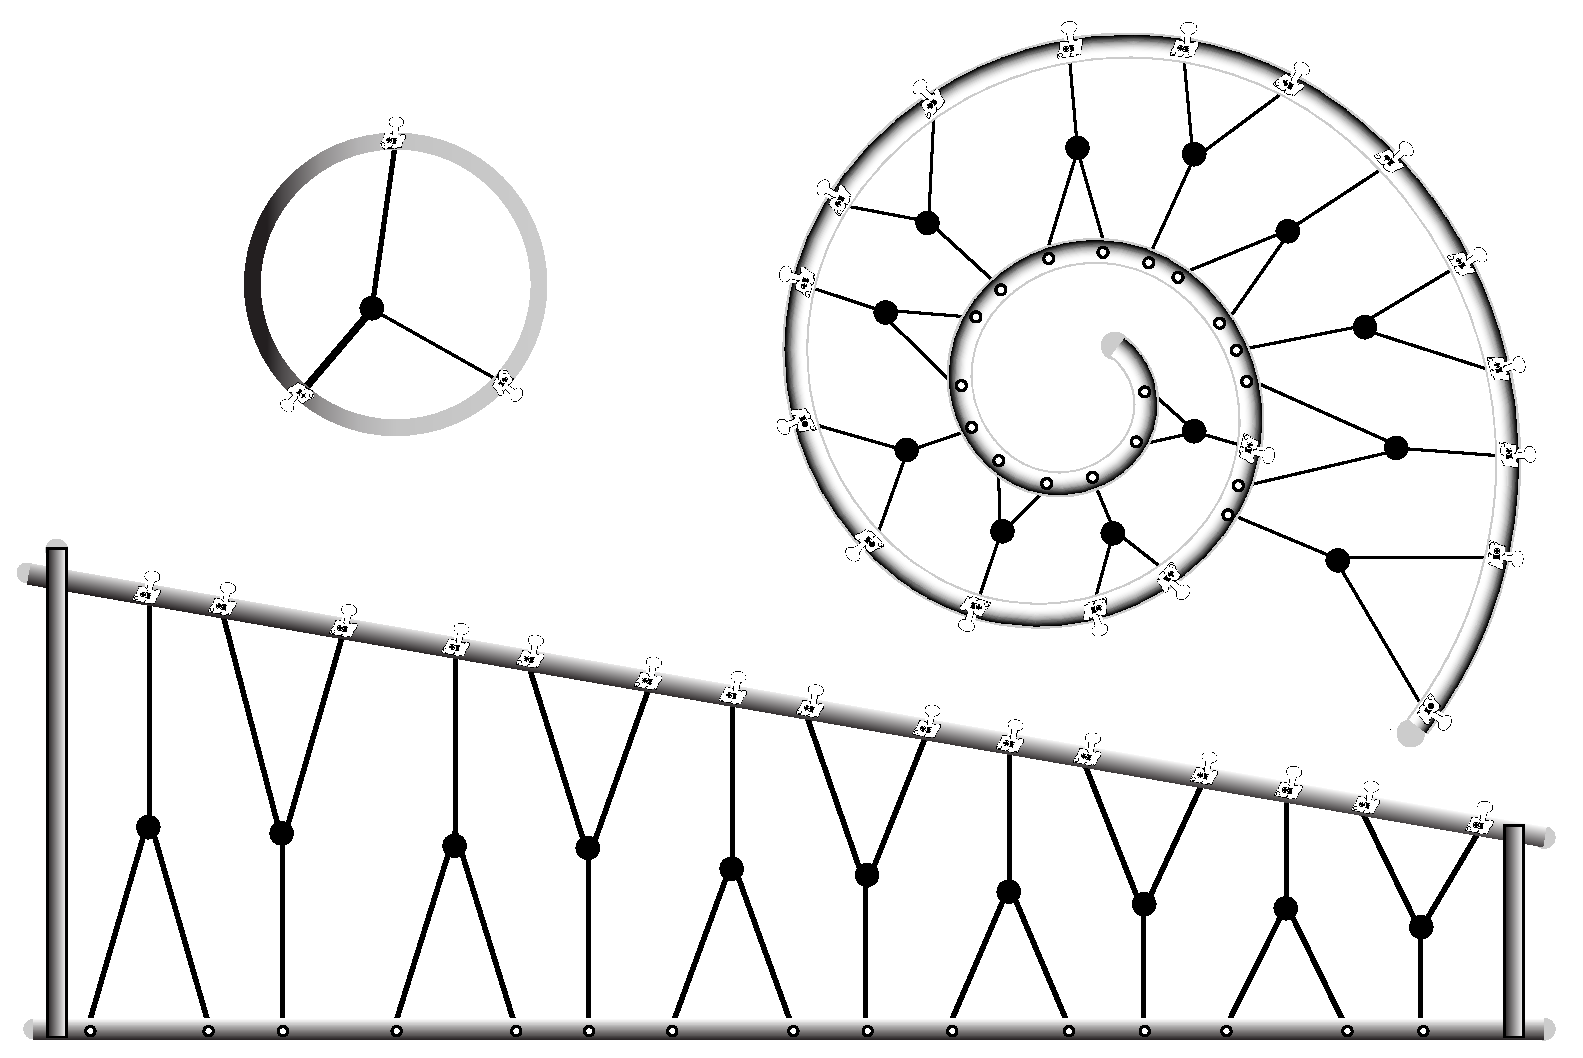
\includegraphics[width=0.5\textwidth]{ArtistsConception.pdf}
\end{frame}
\begin{frame}{Three-String Network}

    \begin{figure}
        \centering
        \includegraphics[width=0.6\textwidth]{HoopArtistsConception.pdf}
        \caption{Parameters: tensions, lengths, mass densities, center mass}
    \end{figure}
\end{frame}



\begin{frame}{The Resonant Frequencies of a Three-String Network Are The Roots of This Equation}
    \begin{align*}
    \scalebox{0.85}{
    $s(\lambda) \equiv \sum_{j=1}^3\sqrt{\tau_j\mu_j} \cos\left(\frac{l_j\sqrt{\mu_j}}{\sqrt{\tau_j}}\lambda\right)\prod_{\substack{k\neq j \\ k=1}}^3 \sin\left(\frac{l_k\sqrt{\mu_k}}{\sqrt{\tau_k}}\lambda\right) + M\lambda \prod_{j=1}^3\sin\left(\frac{l_j\sqrt{\mu_j}}{\sqrt{\tau_j}}\lambda\right)$
    }
    \end{align*}
    
    where: \\
    \medskip
    $l_j$ is the length of the $j^{\text{th}}$ string \\
    \medskip
    $\mu_j$ is the density of the $j^{\text{th}}$ string \\
    \medskip
    $\tau_j$ is the tension of the $j^{\text{th}}$ string \
    medskip
    $M$ is the mass of the center object \\
    \medskip
    \parencite{Brahmi(2019)}
\end{frame}
\begin{frame}{Spectral Graph}
    \begin{figure}
    \centering
    \includegraphics[width=\textwidth,height=.8\textheight,keepaspectratio]{length_5.png}
    \caption{$Parameters: [180, 185, 180, 5, 10, 1, .001, .0015, .001, 0]$ }
    \end{figure}
\end{frame}
\begin{frame}{Spectral Graph}
    \begin{figure}
    \centering
    \includegraphics[width=\textwidth,height=.8\textheight,keepaspectratio]{length_50.png}
    \caption{$Parameters: [180, 185, 180, 50, 10, 1, .001, .0015, .001, 0]$ }
    \end{figure}
\end{frame}
\begin{frame}
    \centering
    \Huge Which values for the tensions, lengths, densities, and center mass be physically achieved?
\end{frame}
\begin{frame}{Newton's Second Law}
    \begin{columns}
        \column{0.5\textwidth}
        \begin{figure}
            \includegraphics[width=\textwidth]{theta_gamma.png}
        \end{figure}
        \column{0.5\textwidth}
 \textbf{Newton's second law in $x$-direction:} \\
        \medskip
        $\tau_1\sin\gamma = \tau_2\sin\theta$\\ 
        \bigskip
        \textbf{Newton's second law in $y$-direction:} \\
        \medskip
        $\tau_3 = \tau_2\cos \theta + \tau_1\cos\gamma$ \\
        \bigskip
    \end{columns}
\end{frame}

\begin{frame}
\frametitle{Values of $\theta$  and $\gamma$ that are physically realistic}
    \centering
    \includegraphics[width=\textwidth,height=.8\textheight,keepaspectratio]{anglediagram1.pdf}
\end{frame}
\begin{frame}
\frametitle{Values of $\theta$  and $\gamma$ that are physically realistic}
    \centering
    \includegraphics[width=\textwidth,height=.8\textheight,keepaspectratio]{anglediagram2.pdf}
\end{frame}
\begin{frame}{Bounds}
    \centering
    \fontsize{24}{28}\selectfont
    % Add Units
    \begin{gather*}
        \theta, \gamma \in [30, 75] \text{\textdegree}\\[0.6cm]
        l_1, l_2, l_3 \in [1, 100] \text{(m)} \\[0.5cm]
        \mu_1, \mu_2, \mu_3 \in [0.001, 1] (\frac{\text{kg}}{\text{m}})\\[0.5cm]
        \text{Center Mass} \in [0, 1] \text{(kg)}
    \end{gather*}
\end{frame}

\begin{frame}{Design Goal}
    \centering
    \Huge Can we design a three-string network such that the first 5 numbers in the ratio spectrum are \{1,3,5,7,9\}?
\end{frame}

\begin{frame}
\frametitle{Hill-Climbing in 2-D}
    \centering
    \includegraphics[width=\textwidth,height=.8\textheight,keepaspectratio]{Optimum.png}
\end{frame}

\begin{frame}
    \centering
    \Huge Simultaneous Perturbation Stochastic Approximation \\ ( SPSA )
\end{frame}


\begin{frame}
\frametitle{SPSA Flowchart}
    \centering
    \includegraphics[width=1.02\textwidth,height=1.4\textheight,keepaspectratio]{Flowchart.png}
\end{frame}
\begin{frame}
\frametitle{SPSA Comparison: Normal vs. Bitmask}

Parameters: $\theta, \gamma, \tau$

Deltas: $\delta = [\delta_\theta, \delta_\gamma, \delta_\tau]$

\begin{table}
\centering
\resizebox{.9\linewidth}{!}{%
\begin{tabular}{|c|c|c|c|}
\hline
\textbf{SPSA Type} & \textbf{$\theta$} & \textbf{$\gamma$} & \textbf{$\tau$} \\
\hline
Normal SPSA & $\theta - \delta_\theta$ & $\gamma - \delta_\gamma$ & $\tau - \delta_\tau$ \\
 & $\theta + \delta_\theta$ & $\gamma + \delta_\gamma$ & $\tau + \delta_\tau$ \\
\hline
Bitmask SPSA & $\theta - \delta_\theta$ & $\gamma - \delta_\gamma$ & $\tau - \delta_\tau$ \\
 & $\theta - \delta_\theta$ & $\gamma - \delta_\gamma$ & $\tau + \delta_\tau$ \\
 & $\theta - \delta_\theta$ & $\gamma + \delta_\gamma$ & $\tau - \delta_\tau$ \\
 & $\theta - \delta_\theta$ & $\gamma + \delta_\gamma$ & $\tau + \delta_\tau$ \\
 & $\theta + \delta_\theta$ & $\gamma - \delta_\gamma$ & $\tau - \delta_\tau$ \\
 & $\theta + \delta_\theta$ & $\gamma - \delta_\gamma$ & $\tau + \delta_\tau$ \\
 & $\theta + \delta_\theta$ & $\gamma + \delta_\gamma$ & $\tau - \delta_\tau$ \\
 & $\theta + \delta_\theta$ & $\gamma + \delta_\gamma$ & $\tau + \delta_\tau$ \\
\hline
\end{tabular}
}
\end{table}

\end{frame}


\begin{frame}
    
\frametitle{Bitmask SPSA Flowchart}
    \centering
    \includegraphics[width=1.02\textwidth,height=1.4\textheight,keepaspectratio]{bitmask_flowchart.png}
\end{frame}

\begin{frame}
\centering\Huge{\Huge{RESULTS}}
\end{frame}
\begin{frame}
\frametitle{Two-Directional - 512 Iterations}
    \begin{figure}
        \centering
        \includegraphics[width=1.1\textwidth,height=2\textheight,keepaspectratio]{Two_512.png}
        \caption{x-axis: iterations, y-axis: spectrum}
    \end{figure}
\end{frame}
\begin{frame}
\frametitle{Bitmask - 2 Iterations}
    \begin{figure}
        \centering
        \includegraphics[width=1.1\textwidth,height=2\textheight,keepaspectratio]{Bitmask_2.png}
        \caption{x-axis: iterations, y-axis: spectrum}
    \end{figure}
\end{frame}
\begin{frame}
\frametitle{Two-Directional - 2560 Iterations}
    \begin{figure}
        \centering
        \includegraphics[width=1.1\textwidth,height=2\textheight,keepaspectratio]{Two_2560.png}
        \caption{x-axis: iterations, y-axis: spectrum}
    \end{figure}
\end{frame}
\begin{frame}
\frametitle{Bitmask - 10 Iterations}
    \begin{figure}
        \centering
        \includegraphics[width=1.1\textwidth,height=2\textheight,keepaspectratio]{Bitmask_10.png}
        \caption{x-axis: iterations, y-axis: spectrum}
    \end{figure}
\end{frame}
\begin{frame}
\frametitle{Two-Directional - 12800 Iterations}
    \begin{figure}
        \centering
        \includegraphics[width=1.1\textwidth,height=2\textheight,keepaspectratio]{Two_12800.png}
        \caption{x-axis: iterations, y-axis: spectrum}
    \end{figure}
\end{frame}
\begin{frame}
\frametitle{Bitmask - 50 Iterations}
    \begin{figure}
        \centering
        \includegraphics[width=1.1\textwidth,height=2\textheight,keepaspectratio]{Bitmask_50.png}
        \caption{x-axis: iterations, y-axis: spectrum}
    \end{figure}
\end{frame}
\begin{frame}
\frametitle{Two-Directional - 128000 Iterations}
    \begin{figure}
        \centering
        \includegraphics[width=1.1\textwidth,height=2\textheight,keepaspectratio]{Two_128000.png}
        \caption{x-axis: iterations, y-axis: spectrum}
    \end{figure}
\end{frame}
\begin{frame}
\frametitle{Bitmask - 500 Iterations}
    \begin{figure}
        \centering
        \includegraphics[width=1.1\textwidth,height=2\textheight,keepaspectratio]{Bitmask_500.png}
        \caption{x-axis: iterations, y-axis: spectrum}
    \end{figure}
\end{frame}
\begin{frame}
\frametitle{Bitmask - 50000 Iterations}
    \centering
    \begin{figure}
        \centering
        \includegraphics[width=1.1\textwidth,height=2\textheight,keepaspectratio]{Bitmask_50000.png}
        \caption{x-axis: iterations, y-axis: spectrum}
    \end{figure}
\end{frame}
\begin{frame}
\frametitle{Expanding our Bounds}
    \centering
    \includegraphics[width=\textwidth,height=.8\textheight,keepaspectratio]{anglediagram2.pdf}
\end{frame}

\begin{frame}
\frametitle{What's Next?}
\Huge{\begin{itemize}
    \item Increasing Bounds
    \item N-String Networks
    \item Different Optimization Algorithms
\end{itemize}}
\end{frame}

\begin{frame}
\centering\Huge{\Huge{Questions?}}
\end{frame}
\begin{frame}{References}
    \begin{enumerate}
        \item S. Goodarzi, "Three-string inharmonic networks", Journal of Mathematics and Music, 2022.
    \end{enumerate}
\end{frame}
\begin{frame}
\frametitle{Root Finding using Chebyshev Polynomials}
    \centering
    \includegraphics[width=\textwidth,height=\textheight,keepaspectratio]{polynomial_fitting.png}
\end{frame}
\begin{frame}{Tension Scaling Law}
    % \textbf{Tension Scaling Law:}
    \Huge{\textbf{If $\tau_i \to r\tau_i$ for $i = 1, 2, 3$ for some $r \in \mathbb{R}^+$, then $\{f_i\} \to \{\sqrt{r} f_i\}$.}}

\end{frame}
\begin{frame}{Tension Ratios}
    \centering
\Huge{
    \[\frac{\tau_1}{\tau_3} = \frac{\sin(\theta)}{\sin(\gamma+\theta)}\]}

    \vspace{.5cm}
\Huge{
    \[\frac{\tau_2}{\tau_3} = \frac{\sin(\gamma)}{\sin(\gamma+\theta)}\]}
\end{frame}
\begin{frame}
\frametitle{Bitmasking}
    \centering
    \includegraphics[width=1.02\textwidth,height=1.4\textheight,keepaspectratio]{bitmasking.png}
\end{frame}
\begin{frame}{Modifying SPSA}
    \begin{itemize}
        \item Use Bitmasks ( 0b000111001 )
        \item Computational Overhead
        \item Potential to converge to answer quicker
        \item Even Further Optimization using Ternary Masks??
    \end{itemize}
\end{frame}
\end{document}
